\section{Hybrid Model}

\begin{frame}{The Hybrid Model: A Synthesis}
	This project introduces a \textbf{novel hybrid model}, combining features from both the Brownian and SDP frameworks.
	
	\vspace{0.5cm}
	\textbf{Core Idea:}
	\begin{itemize}
		\item The stress $X(t)$ evolves stochastically as a \textbf{Brownian process} between glitches (like in Carlin \& Melatos).
		\vspace{0.2cm}
		\item Glitches are triggered \textbf{stochastically} with a state-dependent rate $\lambda(X)$ (like in Fulgenzi et al.).
	\end{itemize}
	
	\vspace{0.3cm}
	This approach models a system where stress accumulation is noisy, and the failure mechanism is probabilistic rather than a hard threshold.
\end{frame}

\begin{frame}{Hybrid Model: Simulation Method}
	The hybrid model requires a \textbf{step-based simulation}, similar to the Brownian model, to handle both the continuous evolution and the probabilistic events.

    \vspace{0.3cm}
    \textbf{Algorithm at each step $\Delta t$:}
	\begin{enumerate}
		\item \textbf{Evolve Stress}: Update the stress level $X$ using the Langevin equation:
		$$ \Delta X = \xi \Delta t + \sigma \sqrt{\Delta t} \cdot N(0,1) $$
		
		\item \textbf{Calculate Glitch Probability}: Determine the instantaneous glitch rate $\lambda(X)$ based on the new stress level. The probability of a glitch in this step is:
		$$ P_{\text{glitch}} \approx \lambda(X) \Delta t $$
		
		\item \textbf{Trigger Glitch?}: Draw a random number $U \sim \text{Uniform}(0,1)$. If $U < P_{\text{glitch}}$, a glitch occurs.
		
		\item \textbf{Reset Stress}: If a glitch occurs, reduce the stress by a random amount $\Delta X_{release}$ drawn from a chosen distribution $\eta(\Delta X | X_{peak})$.
	\end{enumerate}
\end{frame}

\begin{frame}{Hybrid Model: The Master Equation}
	Because it combines a continuous diffusion and state-dependent jumps, its evolution equation is a \textbf{Fokker-Planck equation with a non-local jump term}.

    \vspace{0.3cm}
    For the probability density $p(x, t)$, the equation is:
    \begin{equation}
    \underbrace{\frac{\partial p}{\partial t} = -\frac{\partial}{\partial x}(\xi p) + \frac{\sigma^2}{2}\frac{\partial^2 p}{\partial x^2}}_{\text{Drift-Diffusion (Brownian)}} \underbrace{-\lambda(x)p(x,t) + \int \lambda(y)p(y,t)\eta(x|y)dy}_{\text{Jump Process (SDP)}}
    \end{equation}
    \vspace{0.3cm}

    This equation is complex to solve analytically, making numerical simulations essential to explore the model's behavior.
\end{frame}

\begin{frame}{Hybrid Model: Stress Trajectory}

    \vspace{-0.5em}
	The trajectory shows a \textbf{stochastic ramp-up} due to the Brownian nature, followed by stochastic drops, combining features of both parent models.

    \vspace{-0.5em}
	\begin{figure}
        \centering
        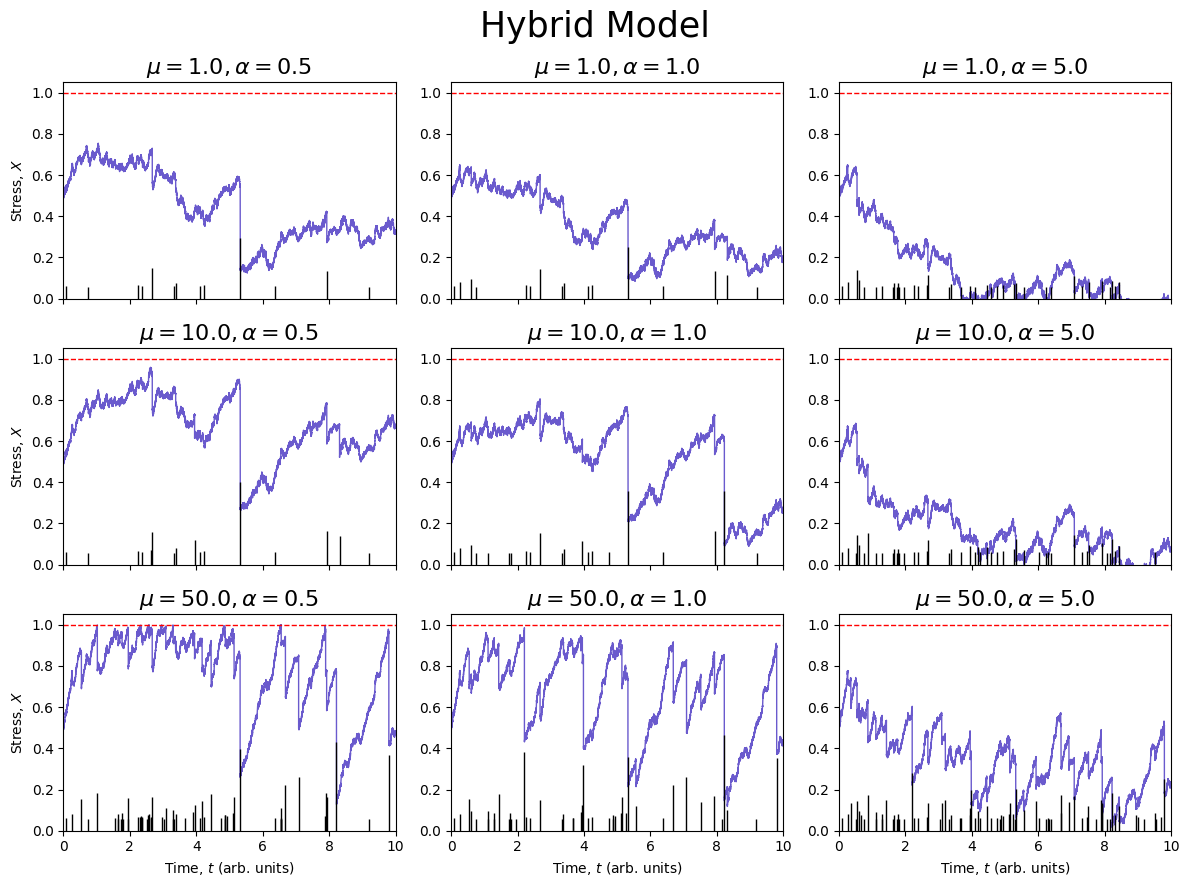
\includegraphics[width=0.79\linewidth,trim={0 0 10 41},clip]{assets/traj_hybrid.png}
        \vspace{-1em}
        \caption{A typical stress trajectory for the Hybrid model.}
    \end{figure}
\end{frame}

\begin{frame}{Hybrid Model: Waiting Time Distribution (Power Law)}

    \begin{itemize}
        \item At \textbf{high $\mu$} and \textbf{high $\alpha$} (drift-dominated, low intrinsic rate), the waiting times are \textbf{exponential-like}.
        \item As \textbf{$\mu$ or $\alpha$ decrease} (more noise or higher rate), the distribution shifts towards a \textbf{power-law}, but with a smoother shape than the pure SDP model.
    \end{itemize}

    \vspace{-0.5em}

    \begin{figure}
        \centering
        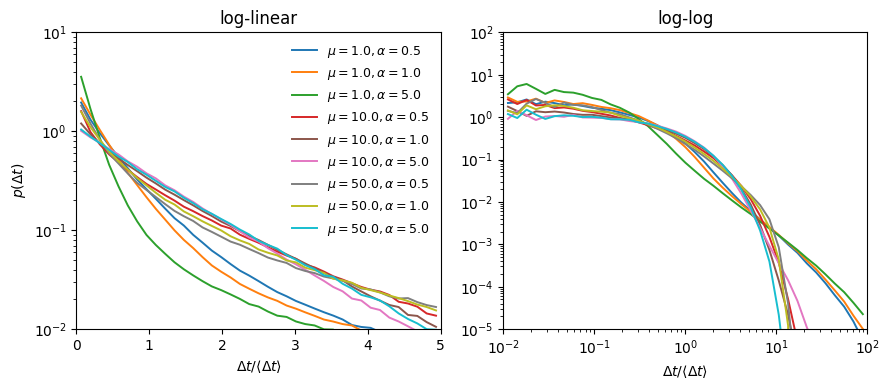
\includegraphics[width=0.9\linewidth]{assets/wtd_powerlaw_hybrid.png}
        \vspace{-1em}
        \caption{$p(\Delta t)$ for hybrid model, power-law $\eta(\Delta X)$, varying $\mu$ and $\alpha$.}
    \end{figure}
\end{frame}

\begin{frame}{Hybrid Model: Waiting Time Distribution (Gaussian)}
    Using a \textbf{Gaussian} glitch size distribution introduces unimodal behavior, similar to the pure Brownian model in the high-drift regime.

    \begin{itemize}
        \item The distribution $p(\Delta t)$ is generally \textbf{unimodal}.
        \item The \textbf{width and skewness} of the distribution depend on the complex interplay between the Brownian noise ($\sigma$) and the SDP rate ($\alpha$).
    \end{itemize}
    \vspace{-0.5em}
    \begin{figure}
        \centering
        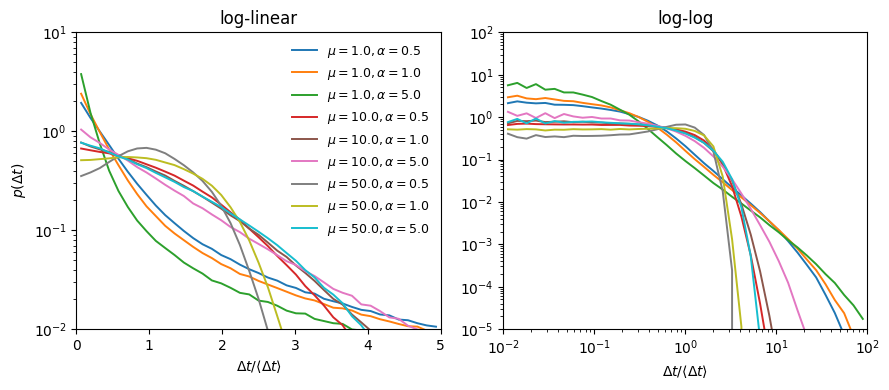
\includegraphics[width=0.85\linewidth]{assets/wtd_gaussian_hybrid.png}
        \vspace{-1em}
        \caption{$p(\Delta t)$ for hybrid model, Gaussian $\eta(\Delta X)$.}
    \end{figure}
\end{frame}

\begin{frame}{Hybrid Model: Waiting Time Distribution (Lognormal)}
    The Lognormal reset distribution confirms the trend observed with the Gaussian case, yielding \textbf{unimodal} waiting time distributions.
    
    \begin{figure}
        \centering
        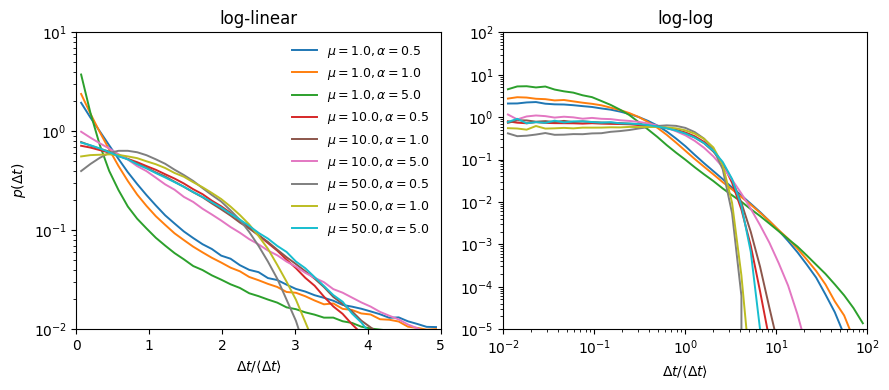
\includegraphics[width=0.85\linewidth]{assets/wtd_lognormal_hybrid.png}
        \vspace{-1em}
        \caption{$p(\Delta t)$ for hybrid model, Lognormal $\eta(\Delta X)$.}
    \end{figure}
\end{frame}